\chapter{Scheduling Conditional Tasks in HEP-Frame}

% *****Pequena intro a existencia de hardware cada vez mais complexo e ao software necessario para usar eficientemente ****
 
 High performance computing platforms have evolved to  support massive amounts of parallelism through the refinement of parallel techniques at an hardware level. This type of techniques includes simultaneous execution of several tasks (on an increasing number of physical cores or processing units, PUs) to the execution of the same task (or sets of instructions) on different data elements (aka known as vector computing). 
 This increasingly complex hardware makes producing code that takes advantages of this functionalities progressively more difficult and cumbersome. For this reasons there is a need to have in mind at all times the hardware specification and capabilities. 
 
%%The increasing complexity of the algorithms and the size of the datasets to be analyzed makes this type of problem computationally intensive and hard to end in a timely manner
% *****Pipelines condicionais *em detalhe e com imagens (e dizer qu eas tarefas sao irregulares) ****

Data analysis applications are typically structured as a sequence of tasks in a pipeline of actions, where data can be modified at each pipeline stage, filtered out and/or output as a result.
The elements that are filtered out are not processed by the next tasks in the pipeline. 
Actions often vary from intensive computing tasks to simple evaluations that may discard irrelevant data. 
In some of this applications decision on some pipeline stages may lead to different alternative solutions, namely different pipeline paths. 
This behaviour will be addressed as conditional pipeline. 
 
 \newpage
\section{Conditional Pipelines}
%entrar detalhe
%imagem pipeline normal vs pipeline multi saida
%levantar questoes de paralelização, escalonamento, eficiencias
Conditional pipelines can be described as a group of tasks that are chained together in which the next tasks to be executed will be decided by the evaluation of a Boolean condition in the current task. 
\begin{figure}[htb!]
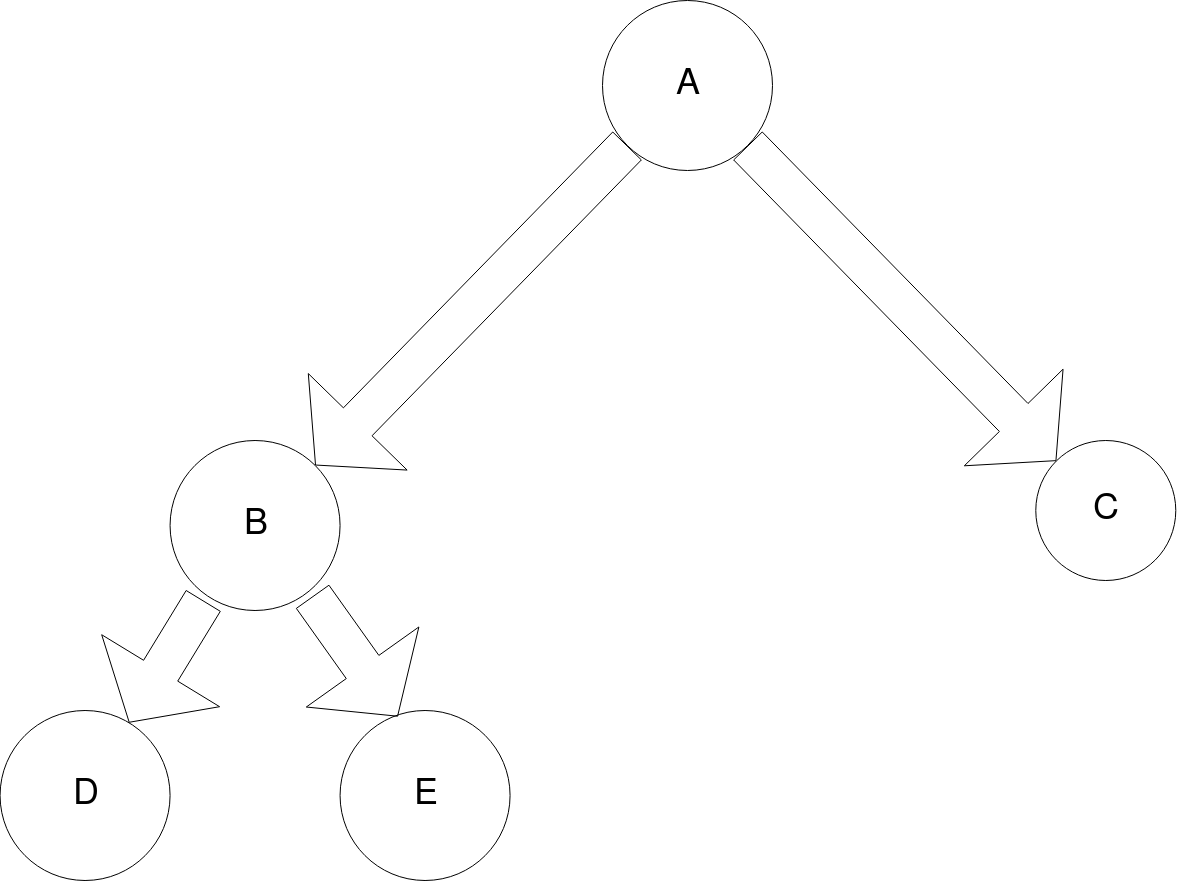
\includegraphics[width=8cm]{latex/img/Named-graph.png}
\qquad
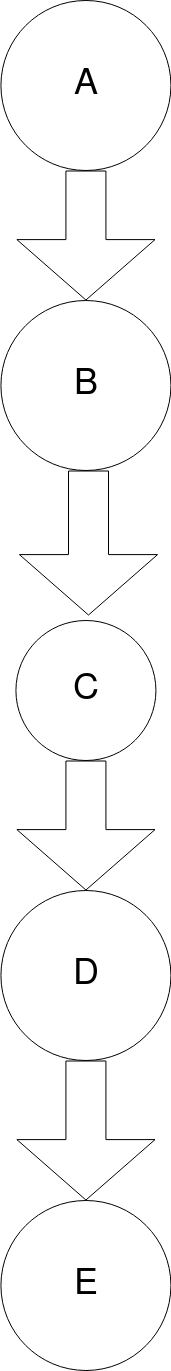
\includegraphics[height=7cm]{latex/img/ClassicPipeline.png}
\captionof{figure}{Conditional pipeline and classical pipeline}
\end{figure}

This means that that in contrary of a normal pipeline where,before any computation the tasks will be processed are already known and in what order they are needed, in a conditional pipelines with all the all the multiple combinations of flows it can only be discovered at run-time for each data-set.
This non deterministic flow introduces questions on parallelism and scheduling for high performance computing, on how can sequential tasks be paralyze that depend on if statement that are known to be problematic for optimizations  and schedule tasks when there is no clue which one is the next to be executed.


\subsection{Graphs to Represent Task Execution Order}
With this multiple tasks that connect with each other in multiple points there is a need to represent them in a structure that can accommodate details needed. 
This will include a way to describe the tasks with the processing part and the control flow part, this is , the computational work that it must execute and the tests that will determine the next task to be executed.
For this type of work the best structure is a graph where vertices represent tasks and edges with a direction associated (directed graph) represent connecting tasks.
When connecting tasks we are also managing dependencies between tasks, by following all the in vertices of a determined task we can determine all the possible previous task that could exist before this one allowing us to create a dependency graph.
With this graph structure we can use the weight on the edges to serve as a weight of the task for the scheduler part of this work, this means that a task with a bigger weight can be more urgent to execute on a speculative execution environment.
Each of this tasks can only be executed one single time to prevent any cycle or deadlock therefore our structure needs to prevent any duplicated execution of a vertex.

\subsection{Conditional Tasks}
In a TEG the vertex represent a conditional task. This is a task that describes the computation part, this is, the data transformation that should be applied to a given data component.
After this the conditional path should be described by a the edges out of this vertex. Each of this edges should be accompanied by a Boolean condition that will determine what is the next task to be executed.
This path choosing should be mutually exclusive, this is, only one of them should be chosen when testing conditions. In the case that more than one of this conditions as a valid outcome then the path with the lowest number vertex should be chosen.
\subsection{Allocation and Scheduling of Conditional Tasks}
With the irregular nature of this tasks and the conditional proposition behaviour there's a very specific set of needs to schedule them in a efficient way.
This means that traditional schedulers based on graphs or lists are not enough because they don't take in count this type of behaviour therefore they are not the most correct to be used in the scheduling of this tasks.
Once that this type of tasks are irregular and there are jumps between tasks to create the flow , there's a chance to try to implement speculative execution that would allows us to pass the challenge of paralyzing the multiple if statements inside of each task.


%\subsection{Computational Efficiency}

%\subsubsection{vector instructions}
%(explicar HW, como tirar partido neste problema)
%\subsubsection{paralelização (dar exemplos de paralelização básica e levantar os problemas com isso)}

%\subsubsection{Multicore}
%\subsubsection{Descrever em detalhe todas as caracteristicas que sao importantes como multiplos cores, caches, vectorizacao, etc}
%\subsubsection{Intel/AMD}

%\subsubsection{Manycore}
%\subsubsection{ARM}

%\section{HEP-Frame and Competitors}




% *****tudo o que precises ou que exista de carater geral desde boost threads, openMP, mpi, tbb, etc ****
 
% *****tudo o que procuraste (descrever o que e e o proposito, de escalonadores, list schedulers (e importante ter alguma coisa e provar que nao e util para o nosso problema, ferammentas DAG, etc, uteis para nos  ****
 
% *****Se calhar uma secao so para falar de grafos (algoritmos para construir e manipular so os que poderao ser uteis) ****




